\documentclass[11pt]{article}

\usepackage{fullpage,graphicx, verbatim, subcaption, amsmath, amssymb}

\title{CSCI 599 Project : Learning the protein coding signature}

\author{Saket Choudhary\\ Team Launchpad \\ skchoudh@usc.edu}

\begin{document}
\maketitle 
\section*{Abstract} 
The central dogma of biology describes how genetic information flows within a system where the RNA is synthesizes from DNA which in turn gets synthesized to proteins. Any gene can be roughly partitioned into three regions: 5' Untranslated Region (UTR), Coding Domain Sequence (CDS) and 3'UTR. While 5'UTR region regulates translation process, the 3'UTR region is involved in post-transcriptional regulation. CDS is the region that codes for protein and is mostly the longest of the three regions. These annotations are available for a lot of organisms, but  not for all organisms even if there genome sequence is completely known. Inferring the protein coding boundaries requires learning the sequence dependencies in the different partitions. Formally, the problem is stated as follows:

\textbf{Input}: A vector $\mathbf{x} \in \mathcal{V}^l$ where $l$ is sequence length  and $\mathcal{V} = \{N, A, C, T, G \}$. where N represents no base and $A,C,T,G$ are the four chemical bases Adenine, Cytosine, Thymine and Guanine.

\textbf{Output}: Labels $\mathbf{y} = \{ \text{5'UTR}, \text{CDS}, \text{3'UTR} \}^l$

In other words, the aim is to be able to first be able to do a base level prediction for one of the three classes and then using a cutoff-length $k$ )to be empirically determined) determine the exact boundaries of these regions.

\section*{Model}
We propose an LSTM based approach to learn these dependencies. The training process would involve training on annotated boundaries of over ~ 25000 genes using the human dataset. 

\section*{Goals}
The project will have two goals, with Goal 2 dependent on Goal 1's success:

\subsection*{Goal 1}
Can the RNN capture the non-random signal in genome? Given a sequence of bases $\{A, C, T, G\}$ can the RNN predict the next base with an accuracy better than a \textit{random} genome? This random genome can consist of a pre-defined length of random permutation of $\{A, C, T, G\}$.

\subsection*{Goal 2}
If Goal 1 is successful, the next goal would be to use this model for a classification problem. Where we predict a label  $\{ \text{5'UTR}, \text{CDS}, \text{3'UTR} \}$ for each base. This will have two parts:
\begin{itemize}
\item Training on human dataset using 15000 genes and testing on remaining ~10000 genes
\item Training on entire human dataset of ~25000 genes and testing on an entirely different organism
\end{itemize}


\begin{figure}[h]
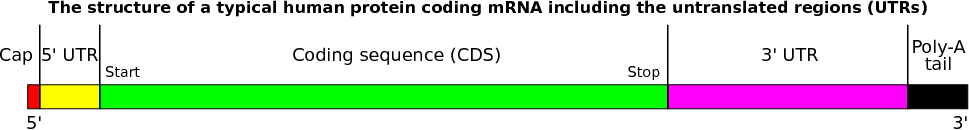
\includegraphics[width=\textwidth]{cds}
\caption{Different regions in a gene.}
\end{figure}
\end{document}
